In this Section, we ablate three design choices: the delay-conditioning mechanism, the target construction scheme, and the degree of left-padding.

\subsection{Ada RMS-Norm} \label{sec:ada-rms}

There are multiple strategies available to incorporate delay conditioning into the model. DSM sums a sinusoidal delay embedding with the combined audio-text embedding. Alternatively, special tokens can be injected in the text stream to indicate the target delay, though this requires repeating the token at sliding-window boundaries. A third approach using Ada RMS-Norm injects the delay into the decoder's residual stream (Section~\ref{sec:lang-dec}).

Figure~\ref{fig:abl-delay-cond} plots WER results for three languages in the FLEURS dataset for the three conditioning methods outlined above. Summing and special tokens perform comparably, whereas Ada RMS-Norm leads to faster convergence and lower overall WER.

\begin{figure*}[t]
    \centering
    \begin{subfigure}[t]{0.32\textwidth}
        \centering
        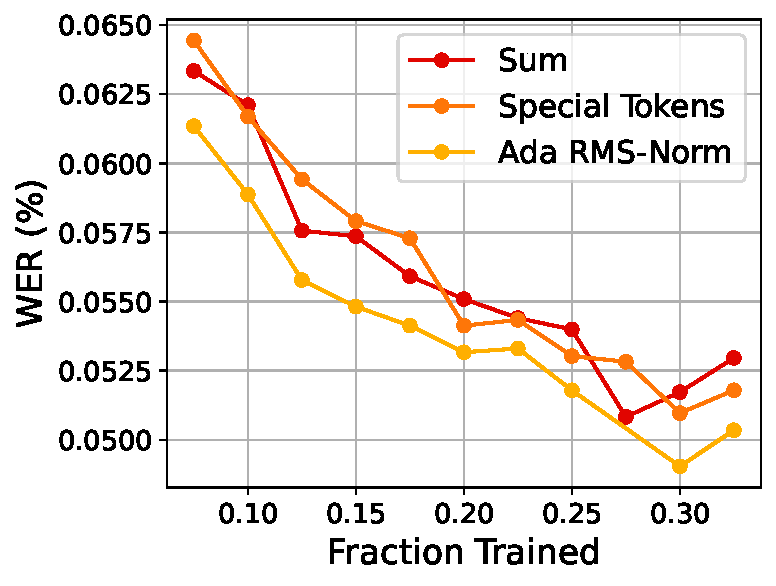
\includegraphics[width=\linewidth]{figures/ablations/time_en.pdf}
        \caption{English}
    \end{subfigure}\hfill
    \begin{subfigure}[t]{0.32\textwidth}
        \centering
        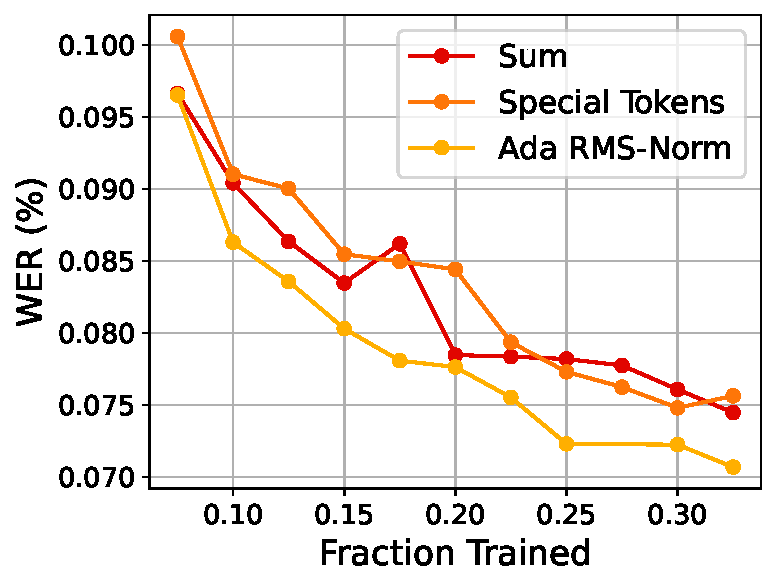
\includegraphics[width=\linewidth]{figures/ablations/time_fr.pdf}
        \caption{French}
    \end{subfigure}
    \begin{subfigure}[t]{0.32\textwidth}
        \centering
        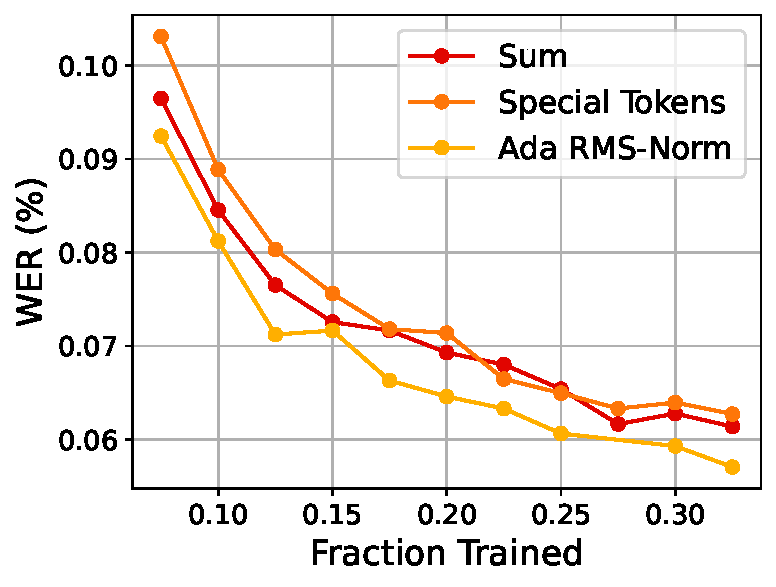
\includegraphics[width=\linewidth]{figures/ablations/time_de.pdf}
        \caption{German}
    \end{subfigure}\hfill
    \caption{\textbf{Ablation of delay-conditioning mechanisms.}
    Word error-rate on three languages from the FLEURS dataset as a function of training progress. Ada RMS-Norm consistently improves convergence speed and final accuracy compared to alternative conditioning strategies.}
    \label{fig:abl-delay-cond}
\end{figure*}


\subsection{Word Grouping} \label{sec:word-grouping}

In Section~\ref{sec:target-construction}, we describe the construction of the target tokens during training. Figure~\ref{fig:abl-target-construction} compares two target schemes: inserting a word-boundary token \texttt{[W]} between consecutive words in the same emission frame, or grouping them without a boundary. Grouping results in much faster convergence and lower overall WERs. It preserves the subword sequences seen during language model pretraining, allowing the decoder to retain its learned text distributions.

\begin{figure*}[t]
    \centering
    \begin{subfigure}[t]{0.32\textwidth}
        \centering
        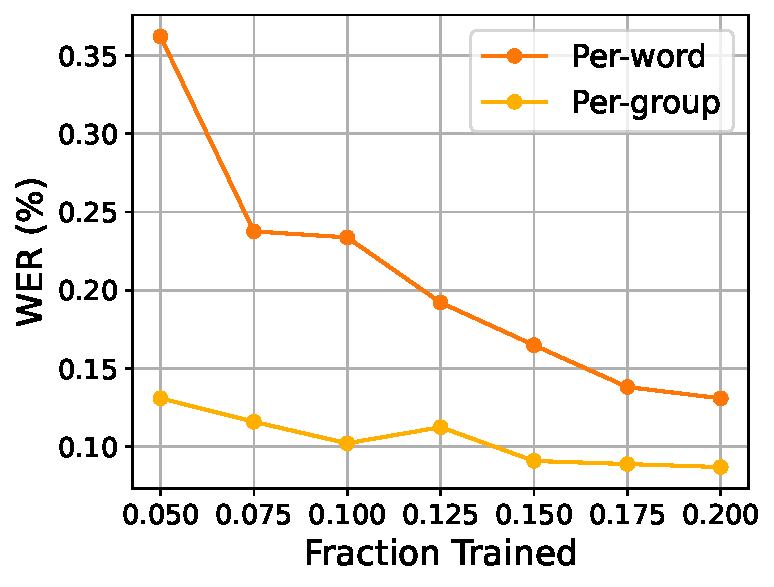
\includegraphics[width=\linewidth]{figures/ablations/group_en.pdf}
        \caption{English}
    \end{subfigure}\hfill
    \begin{subfigure}[t]{0.32\textwidth}
        \centering
        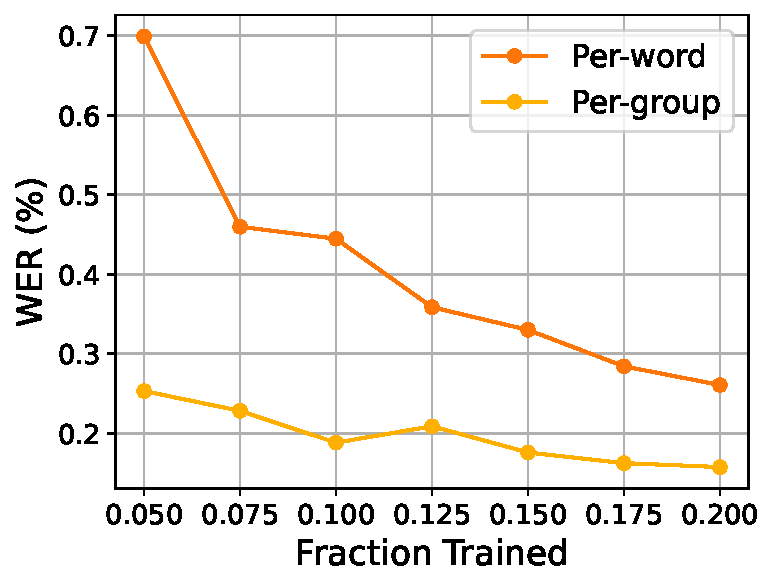
\includegraphics[width=\linewidth]{figures/ablations/group_fr.pdf}
        \caption{French}
    \end{subfigure}
    \begin{subfigure}[t]{0.32\textwidth}
        \centering
        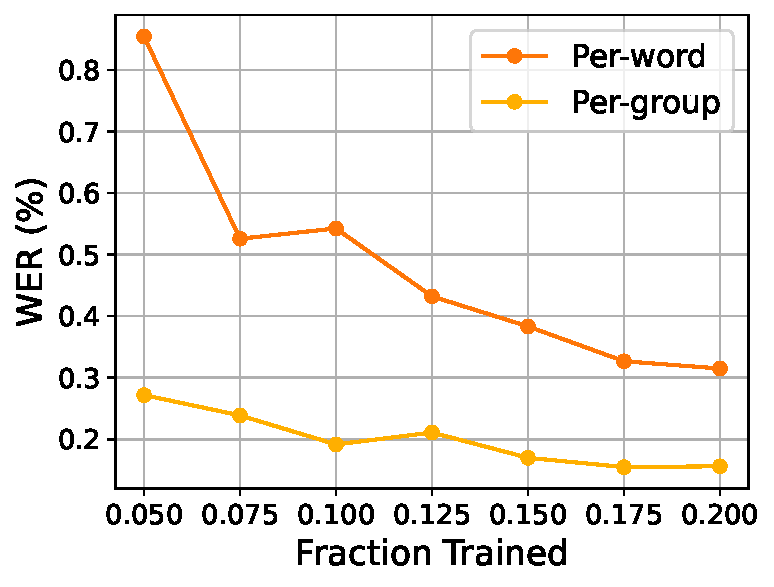
\includegraphics[width=\linewidth]{figures/ablations/group_de.pdf}
        \caption{German}
    \end{subfigure}\hfill
    \caption{\textbf{Ablation of target construction schemes.}
    Word error-rate on three languages from the FLEURS dataset as a function of training progress. Inserting a single word-boundary token \texttt{[W]} per-group better preserves the capabilities of the pre-trained language decoder than inserting a \texttt{[W]} per-word.}
    \label{fig:abl-target-construction}
\end{figure*}

\subsection{Left-Padding}

\looseness=-1 During inference, we explored inserting additional left-padding before the first audio frame. This does not affect streaming delay, as it only increases the size of the prefill step. We pad the audio stream with zeros (equivalent to silence) and the text stream with the corresponding number of \texttt{[P]} tokens.    

Table~\ref{tab:left-padding} shows the WER results across the four benchmark categories as the amount of padding is increased. Increasing the left-padding from 0 to 16 frames improves results across task categories. Further increasing to 32 frames yields additional gains all bar MCV. We hypothesize that left-padding introduces initial tokens that serve a similar role to attention sinks \citep{xiao2024sink}, but leave investigating this to future works.

% We attribute this improvement to providing the model with additional context positions for the earliest audio frames. In standard autoregressive decoding, the first positions lack sufficient prior context for attention to operate effectively. Left-padding introduces initial tokens that serve a similar role to attention sinks \citep{xiao2024sink}: they provide stable positions for the attention mechanism to attend to, preventing the degradation that occurs when the first "real" tokens must also anchor the attention distribution. This is particularly beneficial in streaming, where the model must begin emitting predictions before accumulating substantial context.

\begin{table}[t]
\centering
\caption{\textbf{Effect of left-padding on transcription accuracy.} Macro-average WER (\%) across benchmark categories for different degrees of left-padding.}
\label{tab:left-padding}
\begin{tabular}{ccccc}
\toprule
% & \multicolumn{4}{c}{\textbf{WER (\%)}} \\
% \cmidrule{2-5}
\textbf{Padding Frames} & \textbf{En-Short} & \textbf{En-Long} & \textbf{FLEURS} & \textbf{MCV} \\
\midrule
0 & 9.10 & 10.98 & 9.06 & 16.03 \\
16 & 8.53 & 7.93  & 8.87 & 15.12 \\
32 & 8.47 & 7.73 & 8.72 & 15.24 \\
\bottomrule
\end{tabular}
\end{table}